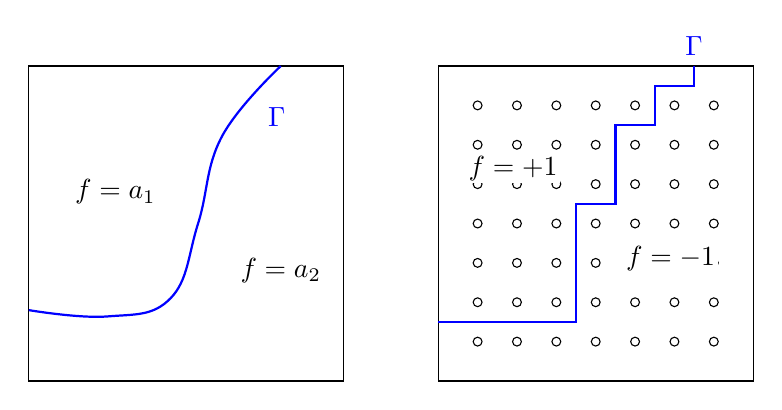
\begin{tikzpicture}[scale=1]
  % continuous segmentation: two regions separated by Gamma
  \draw (0,0) rectangle (4,4);
  \draw[thick,blue] plot[smooth,tension=0.7] coordinates {(0,0.9) (1,0.82) (1.8,1.05) (2.15,2.0) (2.45,3.1) (3.2,4)};
  \node at (1.1,2.4) {$f = a_1$};
  \node at (3.2,1.4) {$f = a_2$};
  \node[blue] at (3.15,3.35) {$\Gamma$};
  % discrete segmentation on a lattice: f = +1 or -1, Gamma a staircase path
  \begin{scope}[xshift=5.2cm]
    \draw (0,0) rectangle (4,4);
    \foreach \i in {0,...,6}
      \foreach \j in {0,...,6}
        \draw (0.5+0.5*\i,0.5+0.5*\j) circle (1.6pt);
    \draw[thick,blue] (0,0.75) -- (1.75,0.75) -- (1.75,2.25) -- (2.25,2.25) -- (2.25,3.25) -- (2.75,3.25) -- (2.75,3.75) -- (3.25,3.75) -- (3.25,4);
    \node[fill=white,inner sep=1pt] at (0.95,2.7) {$f=+1$};
    \node[fill=white,inner sep=1pt] at (2.95,1.55) {$f=-1$};
    \node[blue] at (3.25,4.25) {$\Gamma$};
  \end{scope}
\end{tikzpicture}
